% !TeX encoding = UTF-8
\documentclass[handout,a4paper,t]{beamer}

\usepackage{beamerthemesplit}
\usepackage[utf8]{inputenc}
\usepackage[spanish]{babel}
\usepackage{graphicx}
\usepackage{pstricks} % PSTricks package
\usepackage{setspace}
\usepackage{multirow}
\usepackage{listings}
\usepackage{pgfpages}
\usepackage{hyperref}
\usepackage{etoolbox}
\usepackage{epstopdf}

\makeatletter
\patchcmd{\beamer@sectionintoc}{\vskip1.5em}{\vskip0.5em}{}{}
\makeatother

\setbeamercovered{dynamic}
\setcounter{tocdepth}{2}
\setbeamercolor{frametitle}{fg=black,bg=white}
\setbeamercolor{section in toc shaded}{fg=black}
\setbeamercolor{section in toc}{fg=red}
\setbeamercolor{subsection in toc shaded}{fg=black}
\setbeamercolor{subsection in toc}{fg=red}
\setbeamerfont{section in toc}{size=\small}
\setbeamerfont{subsection in toc}{size=\small}
\setbeamertemplate{section in toc shaded}[default][99]
\setbeamertemplate{subsection in toc shaded}[default][99]

\AtBeginSection[]
{\begin{frame}[c]
  \frametitle{Índice}
	\tableofcontents[currentsection,
        sectionstyle=show/shaded,
        subsectionstyle=hide]
\end{frame}}

\AtBeginSubsection[]
{\begin{frame}[c]
	\frametitle{Índice}
	\tableofcontents[
  		currentsection,
  		sectionstyle=shaded/shaded,
  		currentsubsection,
  		subsectionstyle=show/shaded/hide
		]
\end{frame}}

\setbeamercolor{frametitle}{fg=black,bg=white}

\setbeamertemplate{frametitle}{
	\begin{centering}
		\insertframetitle
		\par
	\end{centering}
}

\usetheme[secheader]{Boadilla}

%% \newcommand{\imp}[1]{{\small{\sf #1}}}

\title[Modelado de Procesos Sw]{Especificación y Modelado de Procesos Software}

\author[P. Sánchez]{\alert{Pablo Sánchez}}

\institute[IIE]{
		   Dpto. Ingeniería Informática y Electrónica \\
		   Universidad de Cantabria \\
		   Santander (Cantabria, España) \\
		   \texttt{sanchezbp@unican.es}
}

\date{}

\begin{document}

\begin{frame}[c]
	\titlepage
	\vspace{-20pt}
	\begin{columns}
		\begin{column}{.1\textwidth}
		\end{column}
		\begin{column}{.4\textwidth}
			\begin{flushleft}
				
\includegraphics[width=.30\textwidth,keepaspectratio=true]{images/istr.eps}
			\end{flushleft}
		\end{column}
		\begin{column}{.5\textwidth}
			\begin{flushright}
				
\includegraphics[width=\textwidth,keepaspectratio=true]{images/logoUC.pdf}
			\end{flushright}
		\end{column}
	\end{columns}
\end{frame}

\begin{frame}[c]
    \frametitle{\alert{Advertencia}}
    \begin{center}
        Todo el material contenido en este documento  no constituye en modo alguno una obra de referencia o apuntes oficiales mediante el cual se puedan preparar las pruebas evaluables necesarias para superar la asignatura. \ \\
        \ \\
        Este documento contiene exclusivamente una serie de diapositivas cuyo objetivo es servir de complemento visual a las actividades realizadas en el aula para la transmisión del contenido sobre el cual versarán las mencionadas pruebas evaluables.  \ \\
        \ \\
        Dicho de forma más clara, \alert{estas transparencias no son apuntes y su objetivo no es en modo alguno servir para que el alumno pueda preparar la asignatura.}
    \end{center}
\end{frame}

\begin{frame}[c]
    \frametitle{Objetivos del Tema}
    \begin{enumerate}[<+->]
         \item Recordar y comprender el concepto de proceso de desarrollo sw.
         \item Conocer y comprender la terminología básica asociada al modelado de procesos de desarrollo sw.
         \item Saber modelar procesos de desarrollo sw en SPEM 2.0.
         \item Saber modelar y crear procesos de desarrollo sw utilizando Eclipse Process Framework.
    \end{enumerate}
\end{frame}

\begin{frame}[c]
    \frametitle{Bibliografía}
    \begin{thebibliography}{1}
    \bibitem{}
    Ian Sommerville.
    \newblock {\em {Software Engineering}}.
    \newblock Addison Wesley, 9 edition, April 2010.

    \bibitem{}
    Object Management~Group (OMG).
    \newblock {\em Software \& Systems Process Engineering Meta-Model Specification 2.0}.
    \newblock OMG Document number: formal/2008-04-01, April 2008.
\end{thebibliography}
\end{frame}

\section{Concepto y Necesidad de los Procesos de Desarrollo Sw}

\subsection{Definición de Proceso Sw}

\begin{frame}[c]
    \frametitle{Proceso de Desarrollo Sw}
    \begin{block}{Proceso de Desarrollo Sw~\cite{sommerville:2010}}
        Un \emph{proceso software} es un conjunto de actividades relacionadas cuyo
        objetivo es la producción de un producto software.
    \end{block}
    \uncover<2->{
    \begin{block}{Proceso de Desarrollo Sw~\cite{ieee:swebok}}
        Un \emph{proceso software} es un conjunto de tareas y actividades relacionadas que
        transforman elementos de trabajo que reciben como entrada en elementos de trabajo
        que devuelven como salida.
    \end{block}
    }
    \uncover<3->{
	\begin{block}{Procesos Software (ISO 12207)~\cite{iso:12207}}
	   Conjunto de actividades interrelacionadas que transforman entradas en salidas.
       Un proceso define quién, qué, cuándo y cómo, para alcanzar un determinado objetivo.
	\end{block}
    }
\end{frame}

\begin{frame}[c]
    \frametitle{Ejemplo de Proceso de Desarrollo Sw}
    \begin{center}
   		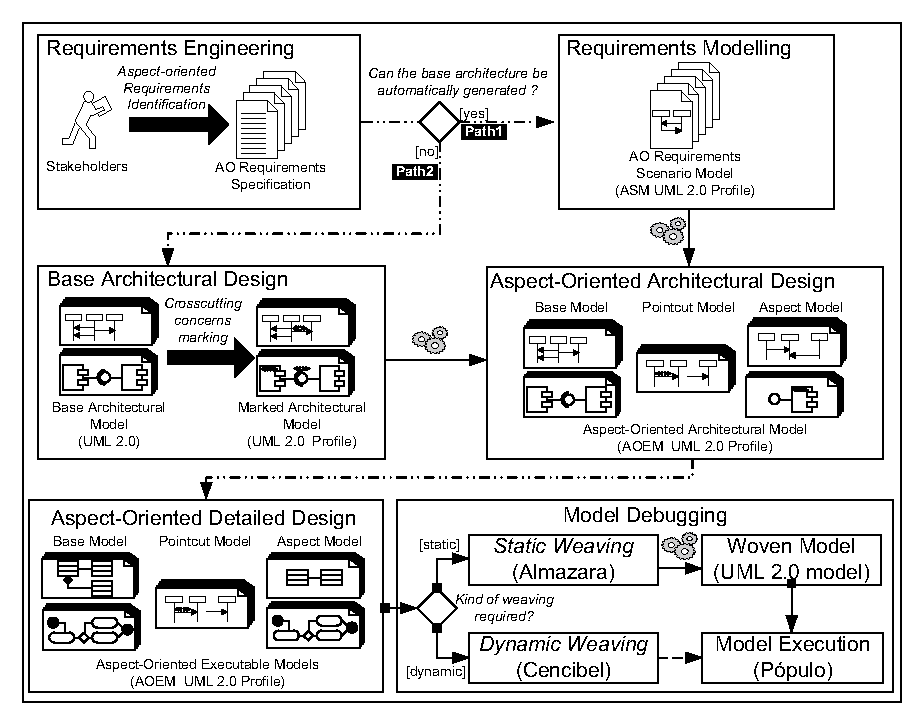
\includegraphics[width=0.75\textwidth,keepaspectratio=true]{images/intro/almadraba.eps}
    \end{center}
\end{frame}

\subsection{Necesidad de los Proceso Sw}

\begin{frame}[c]
    \frametitle{¿Para Qué Sirve Especificar un Proceso de Desarrollo ?}
    \begin{enumerate}[<+->]
        \item Acción No Repetible (\href{http://youtu.be/W77uk1ejcpY}{ver})
        \item Acción Repetible (\href{http://youtu.be/gQ_OHOelPvM}{ver})
    \end{enumerate}
\end{frame}

\begin{frame}[c]
    \frametitle{¿Para Qué Sirve Especificar un Proceso de Desarrollo ?}
    \begin{enumerate}[<+->]
        %%  Sacado de SWEBOK. No tiene explicación. Hay que enrrollarse
        \item Facilitar la comprensión de los procesos de trabajo.
        \item Facilitar la gestión de los procesos de trabajo.
        \item Facilitar la comunicación y coordinación de los equipos de trabajo.
        \item Facilitar el análisis y mejora de los procesos de trabajo.
        \item Facilitar la creación de infraestructura de soporte para dichos procesos de trabajo.
    \end{enumerate}
\end{frame}

\subsection{Elementos Básicos de un Proceso Sw}

\begin{frame}[c]
    \frametitle{Elementos Básicos de un Proceso Sw}
    \begin{center}
		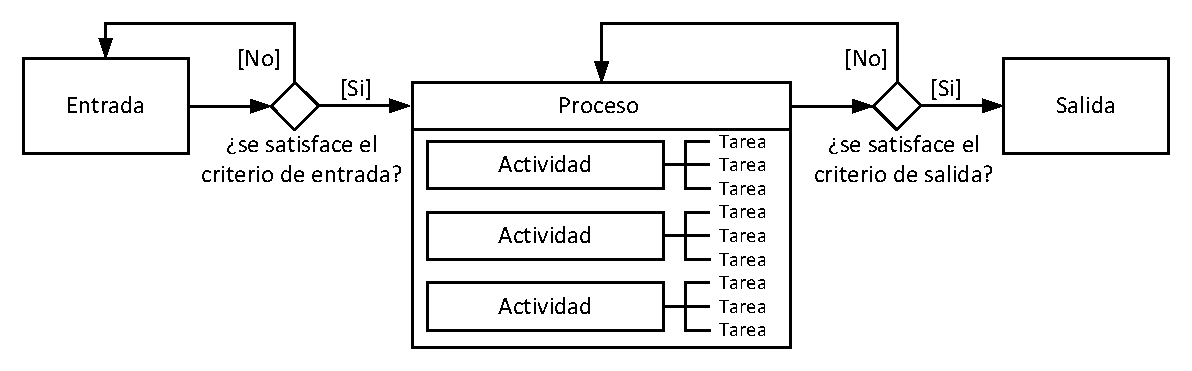
\includegraphics[width=\textwidth,keepaspectratio=true]{images/elements/processElements.eps}
    \end{center}
\end{frame}

%\begin{frame}[c]
%    \frametitle{Elementos Básicos de una Tarea}
%    \begin{enumerate}[<+->]
%        \item Roles
%        \item Técnicas
%        \item Herramientas
%        \item Capacidades
%        \item Recursos
%        \item Medidas para Análisis de Rendimiento
%    \end{enumerate}
%\end{frame}

\subsection{Fases Habituales de un Ciclo de Vida Sw}

\begin{frame}[c]
    \frametitle{Fases Típicas de un Proceso de Desarrollo Sw}
    \begin{center}
        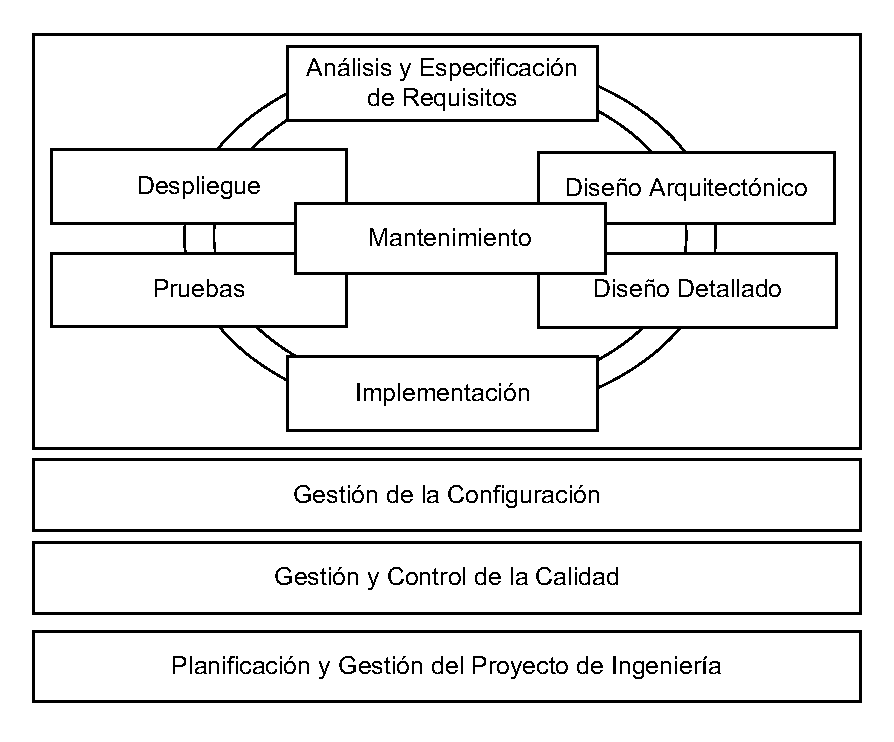
\includegraphics[width=0.75\textwidth,keepaspectratio=true]{images/intro/cicloVidaSw.eps}
    \end{center}
\end{frame}

\section{Tipos Básicos de Metodologías Sw}

\subsection{Metodologías Ágiles y Pesadas}

\begin{frame}[c]
    \frametitle{Índice}
    \begin{enumerate}
         \item Concepto y Necesidad de los Procesos de Desarrollo Sw
         \item \alert{Tipos Básicos de Metodologías Sw}
         \begin{enumerate}
             \item \alert<2->{Metodologías Ágiles y Pesadas}
             \item Ejemplos de Metodologías
        \end{enumerate}
        \item Modelado de Procesos de Desarrollo con SPEM 2.0
        \item Sumario y Referencias
    \end{enumerate}
\end{frame}

\begin{frame}[c]
    \frametitle{Metodologías Pesadas y Ágiles}
    \begin{block}{Metodologías Pesadas o Rígidamente Planificadas}
        Se basan en la definición de un plan de trabajo al cual debemos de adherirnos
        y que es complejo o difícil de cambiar. Suele tener roles y procesos claramente
        definidos.
    \end{block}
    \uncover<2->{
    \begin{block}{Metodologías Ágiles}
        Se basan en una organización del trabajo que permita la definición de planes de trabajo, procesos y productos fácilmente modificables en función de las demandas de los usuarios, con los cuales se debe mantener un permanente contacto, y al cual se le deben proporcionar versiones parciales y operativas del software con frecuencia.
    \end{block}
    }
\end{frame}

\begin{frame}[c]
	\frametitle{Manifiesto Ágil}
	\begin{enumerate}[<+->]
		\item Personas y trato personal sobre procesos y herramientas.
		\item Software que funcione antes que extensos modelos software.
		\item Colaboración con el cliente frente a renegociaciones de contrato.
		\item Ser capaz de responder al cambio antes que seguir un plan fijo.
	\end{enumerate}
\end{frame}

\begin{frame}[t]
	\frametitle{Principios del Manifiesto Ágil}
	\begin{enumerate}[<+->]
		\item Satisfacción del cliente mediante entregas tempranas y continuas de software evaluable.
		\item Los cambios son siempre bien recibidos.
		\item Entregar software operativo frecuentemente.
		\item Gestores y programadores deben trabajar juntos a diario.
		\item Para construir software hacen falta trabajadores motivados.
		\item La mejor forma de proporcionar información es cara a cara.
		\item El principal indicador del avance de un proyecto es la cantidad de software operativo que se ha construido.
		\item El desarrollo software debería ser abordable.
		\item La excelencia técnica y los buenos diseños facilitan la agilidad.
		\item La simplicidad es primordial.
	\end{enumerate}
\end{frame}

\subsection{Ejemplos de Metodologías}

\begin{frame}[t]
    \frametitle{Desarrollo en Cascada}
	\rput[lt](2.5,0){
	   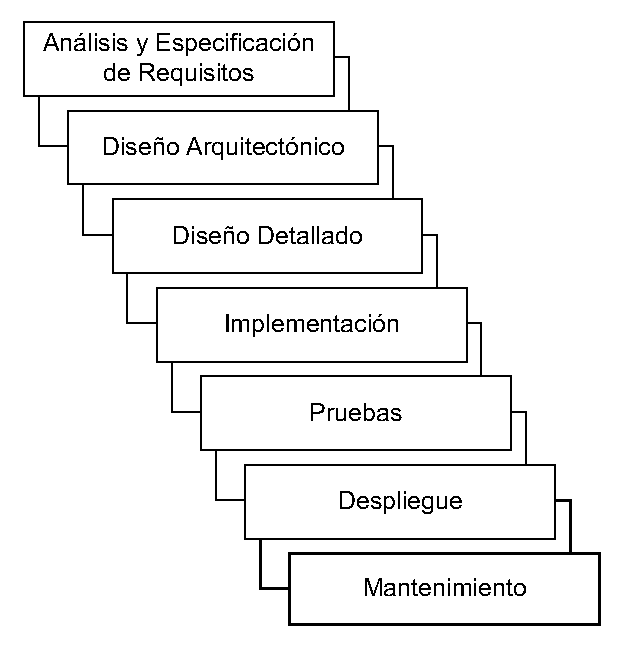
\includegraphics[width=7cm,keepaspectratio=true]{images/modelos/cascada.eps}
	}
\end{frame}

\begin{frame}[t]
    \frametitle{Desarrollo Iterativo o Incremental}
	\rput[lt](1,0){
	   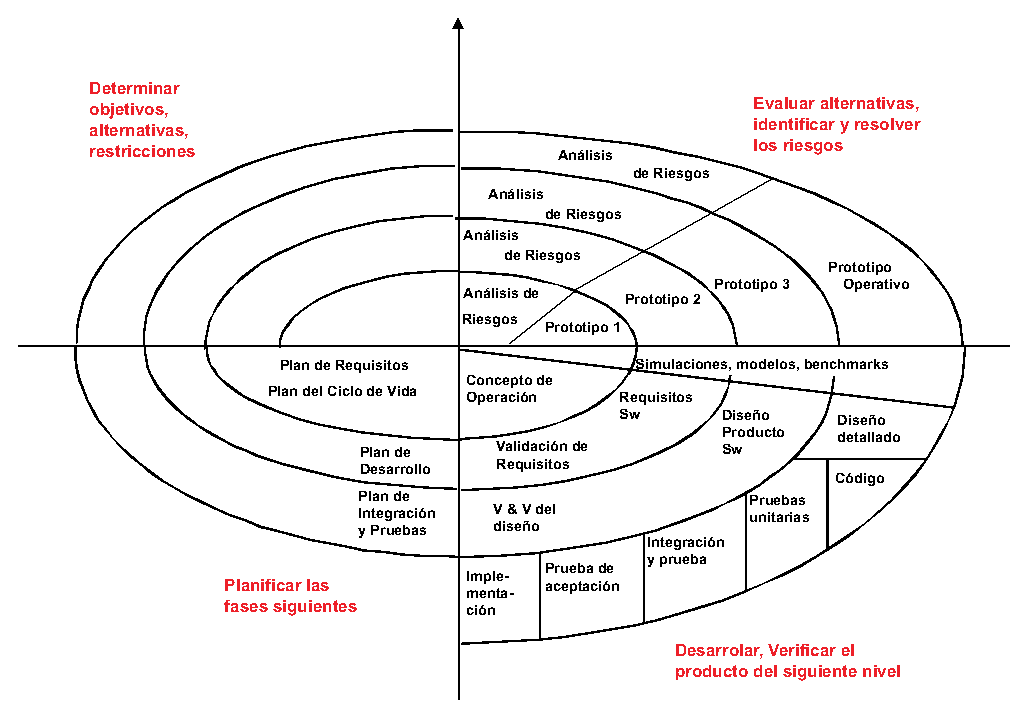
\includegraphics[width=10cm,keepaspectratio=true]{images/modelos/espiral.eps}
	}
\end{frame}

\begin{frame}[t]
    \frametitle{Desarrollo Basado en Reutilización}
	\rput[lt](1,0){
	   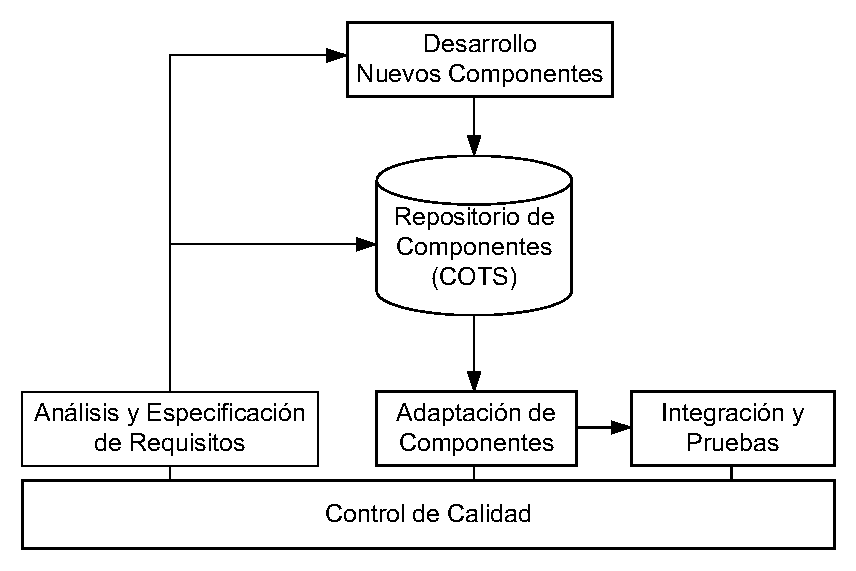
\includegraphics[width=10cm,keepaspectratio=true]{images/modelos/componentes.eps}
	}
\end{frame}

\begin{frame}[t]
    \frametitle{Métodos Formales}
	\rput[lt](1,0){
	   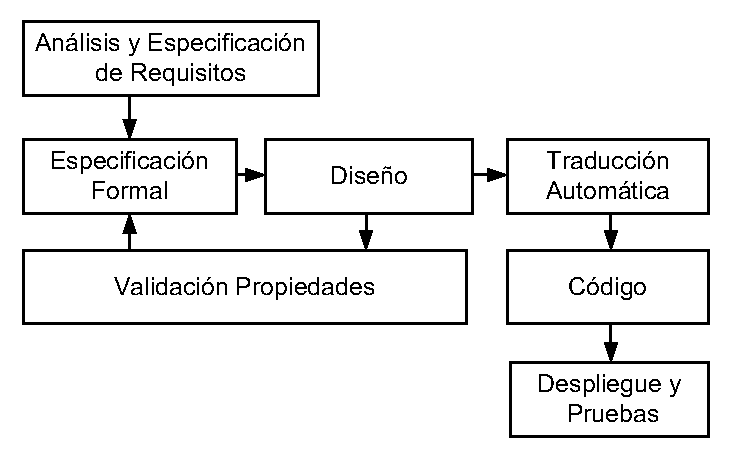
\includegraphics[width=10cm,keepaspectratio=true]{images/modelos/sintesis.eps}
	}
\end{frame}

\section{Modelado de Procesos de Desarrollo con SPEM 2.0}

\subsection{Introducción}

\begin{frame}[c]
    \frametitle{SPEM 2.0}
    \begin{block}{Software and Systems Process Engineering Metamodel (SPEM) 2.0}
        SPEM es un lenguaje de modelado cuyo objetivo es permitir la especificación de procesos de desarrollo de software y sistemas~\cite{spem:2008}.
    \end{block}
\end{frame}

\begin{frame}[c]
    \frametitle{Objetivos SPEM 2.0}
    \begin{enumerate}[<+->]
        \item Permitir el desarrollo, gestión y mantenimiento de la especificación de procesos de desarrollo.
        \item Proporcionar contenidos reutilizables, alojados en librerías bien definidas y estandarizadas, para la definición de metodologías de desarrollo.
        \item Permitir la especificación de procesos de desarrollo a partir de la configuración de elementos preexistentes.
        \item Favorecer la implantación y consolidación de los procesos de desarrollo especificados.
    \end{enumerate}
\end{frame}

\begin{frame}[c]
    \frametitle{Esquema General Funcionamiento SPEM 2.0}
    \begin{center}
        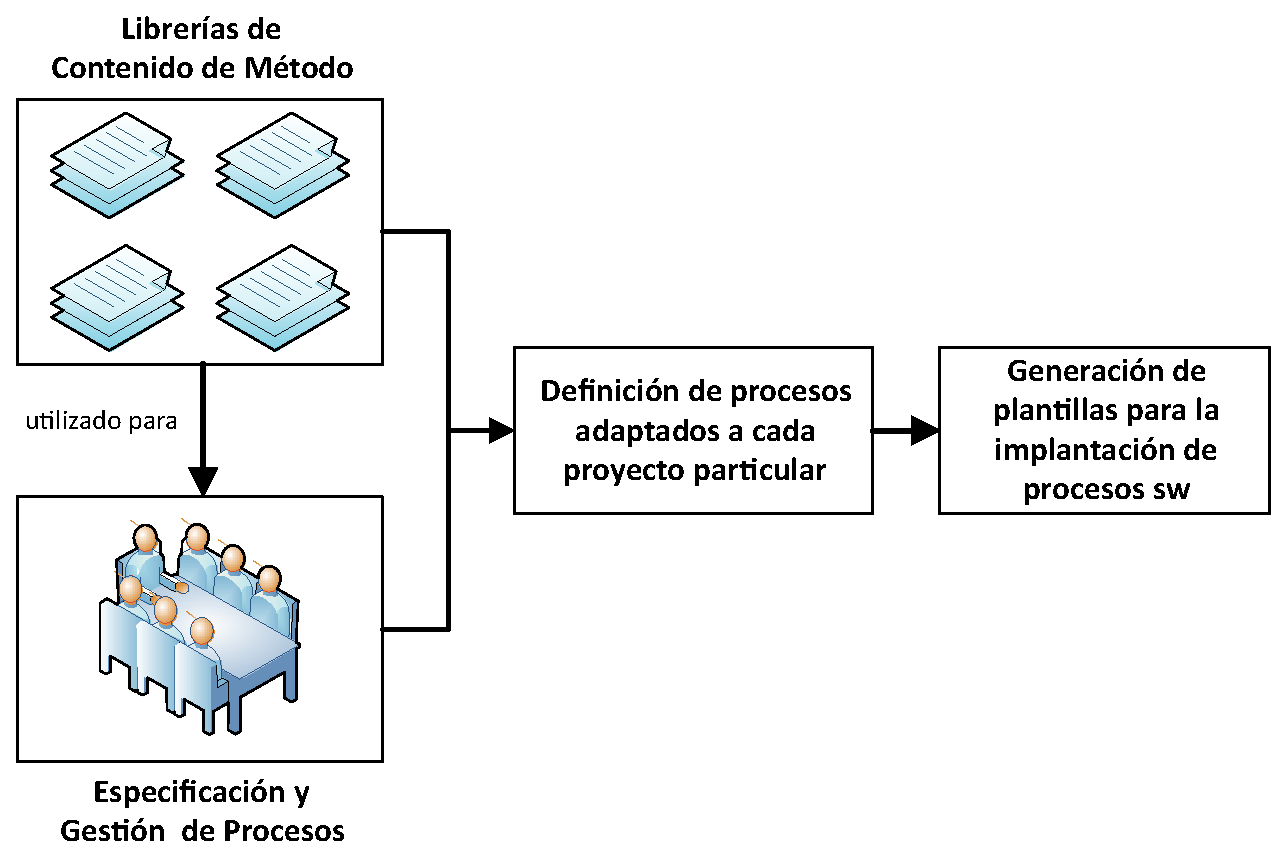
\includegraphics[width=0.90\textwidth,keepaspectratio=true]{images/spem/spemOverview.eps}
    \end{center}
\end{frame}

\begin{frame}[c]
    \frametitle{Características SPEM 2.0}
    \begin{enumerate}[<+->]
        \item Separación de la definición y aplicación de los contenidos de un proceso de desarrollo.
        \item Gestión consistente de variaciones de procesos de desarrollo.
        \item Soporte para múltiples ciclos de vida.
        \item Soporte para la especificación y personalización de elementos variables.
        \item Definición de patrones de procesos para la definición de procesos de desarrollo por instanciación y ensamblado de patrones.
        \item Soporte para la definición de elementos de un proceso de desarrollo como componentes de caja negra.
    \end{enumerate}
\end{frame}

\subsection{Elementos de Contenido}

\begin{frame}[c]
    \frametitle{Elementos de Contenido SPEM 2.0}
    \begin{description}[<+->]
        \item[Qualification] Representa una determinada habilidad o competencia.
        \item[Rol Definition] Especifica un conjunto de habilidades, competencias y responsabilidad, tanto de una persona como de un grupo de personas.
        \item[Task Definition] Describe una unidad de trabajo que deberá ser realizada por uno o más roles.
        % Granularidad: varias horas o días
        \item[Step] Especifica una acción (normalmente indivisible y consistente) del trabajo que debe ser realizado para completar una tarea.
        \item[Tool Definition] Especifica las capacidades que debe poseer una herramienta para dar soporte a ciertas definiciones de roles en la realización de ciertas definiciones de tareas.
        \item[Work Product Definition] Elementos tangibles que son producidos, consumidos o modificados por las tareas.
        \item[Guidance] Elementos que proporciona información complementaria a otros elementos.
    \end{description}
\end{frame}

\begin{frame}[c]
    \frametitle{Elementos Organizativos de SPEM 2.0}
    \begin{description}[<+->]
        \item[Category] Elemento utilizado para clasificar contenidos de acuerdo al criterio del usuario.
        \item[Method Plug-in] Contenedor de elementos reutilizables para la definición de contenidos y procesos de métodos de desarrollo sw.
        \item[Method Configuration] Colección de plug-ins de los cuales se ha seleccionado parte de su contenido.
        \item[Method Library] Contenedor que aloja tanto \emph{Method Plug-in}s como \emph{Method Configurations}
    \end{description}
\end{frame}

\subsection{Elementos Predefinidos}

\begin{frame}[c]
    \frametitle{Elementos de Trabajo Predefinidos en SPEM 2.0}
    \begin{description}[<+->]
        \item[Artifacts] Productos de trabajo tangibles que son consumidos o producidos por una tarea.
        \item[Deliverable] Producto de trabajo que posee cierto valor para un cliente o \emph{stakeholder}.
        \item[Outcome] Productos de trabajo intangibles, que muestran un resultado o estado.
    \end{description}
\end{frame}

\begin{frame}[c]
    \frametitle{Elementos de Asistencia Predefinidos en SPEM 2.0 (I)}
    \begin{description}[<+->]
        \item[Checklist] Conjunto de items que necesitan ser completados o verificados.
        \item[Concept] Pequeño manual o tutorial que describe un concepto relacionado con uno o más elementos de un proceso de desarrollo.
        \item[Estimate] Proporciona medidas, o procedimientos de medida, para estimar el esfuerzo asociado a una cierta tarea, así como instrucciones para su interpretación.
        \item[Estimating Metric] Métrica utilizada para medir esfuerzos asociados a un elemento.
        \item[Estimation Considerations] Indicaciones acerca de cómo aplicar métricas dentro de un proyecto concreto.
        \item[Example] Ejemplo de un producto o tarea.
    \end{description}
\end{frame}

\begin{frame}[c]
    \frametitle{Elementos de Asistencia Predefinidos en SPEM 2.0 (II)}
    \begin{description}[<+->]
        \item[Guideline] Proporciona detalles acerca de cómo realizar una determinada tarea o tareas o cómo elaborar un elemento o elementos de trabajo.
        \item[Practice] Estrategia de eficacia probada para la realización de una tarea de impacto positivo el la calidad de los productos o del proceso.
        \item[Report] Plantilla predefinida que contiene información automáticamente generada sobre diversos elementos de trabajos.
        \item[Reusable Asset] Solución a un problema dentro de un contexto determinado.
        \item[Roadmap] Representa la ejecución lineal de una actividad o proceso.
    \end{description}
\end{frame}

\begin{frame}[c]
    \frametitle{Elementos de Asistencia Predefinidos en SPEM 2.0 (II)}
    \begin{description}[<+->]
        \item[Template] Proporciona un documento plantilla para la elaboración de elementos de trabajo.
        \item[Term Definition] Define conceptos que se integran en el glosario.
+
        \item[Tool Mentor] Tutorial acerca de cómo utilizar una determinada herramienta para ejecutar un determinado trabajo.
        \item[Whitepaper] Son descripciones de conceptos que han sido revisados por entidades externas.
        \item[Supporting Material] Categoría donde se clasifican todos los elementos de asistencia que no encajan en ninguna de las categorías anteriores.
    \end{description}
\end{frame}

\begin{frame}[c]
    \frametitle{Categorías Predefinidas en SPEM 2.0}
    \begin{description}[<+->]
        \item[Discipline] Conjunto de tareas relacionadas dentro de un área de mayor nivel dentro de un proyecto sw.
        \item[Role Set] Contenedor para definición de roles.
        \item[Domain] Conjunto de elementos de trabajo relacionados por algún tipo de afinidad.
        \item[Tool Category] Contenedor para los tutoriales de herramientas.
    \end{description}
\end{frame}

\begin{frame}[c]
    \frametitle{Procesos Predefinidos en SPEM 2.0}
    \begin{description}[<+->]
        \item[Delivery Process] Describe un proceso sw completo que termina con la entrega de un sistema.
        \item[Phase] Representa un periodo de importancia dentro de un proyecto, cuya finalización genera productos o actividades relevantes.
        \item[Iteration] Conjunto de actividades que se repiten más de una vez.
        \item[Capability Pattern] Conjuntos reutilizables de actividades que se utilizan para crear procesos.
        \item[Process Planning Template] Proceso que está preparado para su integración con una herramienta de gestión de proyectos.
    \end{description}
\end{frame}

\subsection{Mecanismos de Variabilidad}

\begin{frame}[c]
    \frametitle{Variabilidad de los Contenidos de Método en SPEM 2.0}
    \begin{description}[<+->]
        \item[Contributes] Añade propiedades a un elemento ya existente, que resulta modificado dentro de una configuración.
        \item[Replaces] Reemplaza propiedades de un elemento ya existente, que resulta modificado dentro de una configuración.
        \item[Extends] Hereda de un elemento ya existente. El elemento hijo puede añadir nuevos elementos, pero el padre se conserva intacto.
        \item[Extends and Replace] Reemplaza las propiedades que se especifiquen como nuevas de un objeto ya existente, que resulta modificado dentro de una configuración. Las propiedades no especificadas se conservan, como si se hubiesen heredado.
    \end{description}
\end{frame}

\subsection{Definición de Procesos}

\begin{frame}[c]
    \frametitle{Terminología de Gestión de Proyectos}
    \begin{block}{Hito}
        Una \emph{hito} (o \emph{milestone}) es un evento de importancia dentro de del desarrollo de un proyecto.
    \end{block}
    \uncover<2->{
    \begin{block}{Estructura de Descomposición de Trabajos}
        Una \emph{Estructura de Descomposición de Trabajos}, o \emph{Work Breakdown Structure (WBS)}, es una descomposición jerárquica  de un proyecto en actividades y subactividades que identifica los hitos y artefactos generados por estas actividades.
    \end{block}
    }
\end{frame}

\begin{frame}[c]
    \frametitle{Propiedades de los Elementos de un Proceso en SPEM 2.0}
    \begin{description}[<+->]
        \item[hasMultipleOcurrences] El elemento puede aparecer varias veces en una WBS final.
        \item[isRepeteable] El elemento puede aparecer varias veces en una WBS final; y sus ejecuciones son secuenciales.
        \item[isOptional] La inclusión del WBS cuando se instancia el proceso es opcional.
        \item[isOngoing] Representa tareas rutinarias y repetitivas.
        \item[isEventDriven] Su comienzo está asociado a la ocurrencia de un cierto evento.
    \end{description}
\end{frame}

\begin{frame}[c]
    \frametitle{Elementos de Procesos SPEM 2.0}
    \begin{description}[<+->]
        \item[Role Use] Representa la ocurrencia de una persona concreta dentro de una actividad, desempeñando un determinado rol.
        \item[Work Use] Representa la ocurrencia de un elemento de trabajo dentro de una actividad, ya sea como parámetro de entrada, de salida o como mero participante.
        \item[Activity] Representa una unidad de trabajo asignable a personas concretas representadas por utilizaciones de rol.
    \end{description}
\end{frame}

\section{Sumario y Referencias}

\subsection{Sumario}

\begin{frame}[c]
    \frametitle{¿Qué Tengo que Saber de Todo Esto?}
    \begin{enumerate}[<+->]
        \item Conocer y comprender la importancia de definir procesos de desarrollo sw.
        \item Ser capaz de utilizar la terminología asociada a la definición de procesos de desarrollo sw.
        \item Conocer y comprender en qué consiste cada etapa de un ciclo de vida sw.
        \item Conocer y comprender las principales tipos de metodologías de desarrollo.
        \item Ser capaz de utilizar SPEM 2.0 para definir procesos de desarrollo sw.
    \end{enumerate}
\end{frame}

\subsection{Referencias}

\begin{frame}
	\frametitle{Referencias}
	\bibliographystyle{apalike}
    \bibliography{metodos}
\end{frame}

\end{document}
